\section{Your Proposed Method}\label{sec:yourmethod}
In this section we propose an optimized implementation of the quantization and Quantized Matrix-Matrix Multiplication (QMMM) functions introduced in \cref{sec:background} that uses four bits compression. We start by presenting the data structure that we use for our baseline implementation. We continue by analysing the bottlenecks of this implementation and by proposing a set of solutions to achieve a higher performance.

\mypar{Baseline implementation}
We presented the algorithm at the base of a straight forward implementation of a simple QNN using a $k$-bits compression scheme in \cref{sec:background}. Here we introduce the data structure necessary to a naive implementation in case $k=4$. Using a 4-bits compression scheme presents challenges due to the byte addressability of the computer memory and to the lack of a built-in 4-bits integer data type. As a consequence, we have to define our custom data structure. One way of operating on entities that require less than a byte for storage is to use structs in combination with bit fields. Nevertheless, byte addressability of the memory does not make it possible to load or store less than one byte at a time. Hence, using bit fields to define a custom data type that stores a single 4-bits integer is wasteful.  In the proposed solution we define the $uint4x4\_t$ data structure. This is a 2 bytes struct that exploits bit fields to store four integers of 4 bits each. The reason why we pack four integers in one struct instead of two is because it allows us to define a data type that is more convenient for QMMM. Given a $n\times m$ weight matrix $\mathbf{A}$ of floats, its 4-bits quantized counterpart $\tilde{\mathcal{Q}}(\mathbf{A})$ is stored as an $\frac{n}{2}\times \frac{m}{2}$ matrix of $uint4x4\_t$. Because of this design choice, we assume both $n$ and $m$ to be even. In particular, the element $(i, j)$ of $\tilde{\mathcal{Q}}(\mathbf{A})$ contains the quantized representation of the elements of $\mathbf{A}$ at the following indices: $(2i, 2j),~(2i, 2j+1),~(2i+1, 2j),~(2i+1, 2j+1)$. The relation between the logical layout and the memory layout for the original matrix $\mathbf{A}$ and its quantized version that uses $uint4x4\_t$ data structure,   $\tilde{\mathcal{Q}}(\mathbf{A})$, can be seen in \cref{fig:uint4x4_t}. The difference between the memory layout of the $\mathbf{A}$ and $\tilde{\mathcal{Q}}(\mathbf{A})$ will play an important role in the vectorization of the code.


\begin{figure}
\centering
  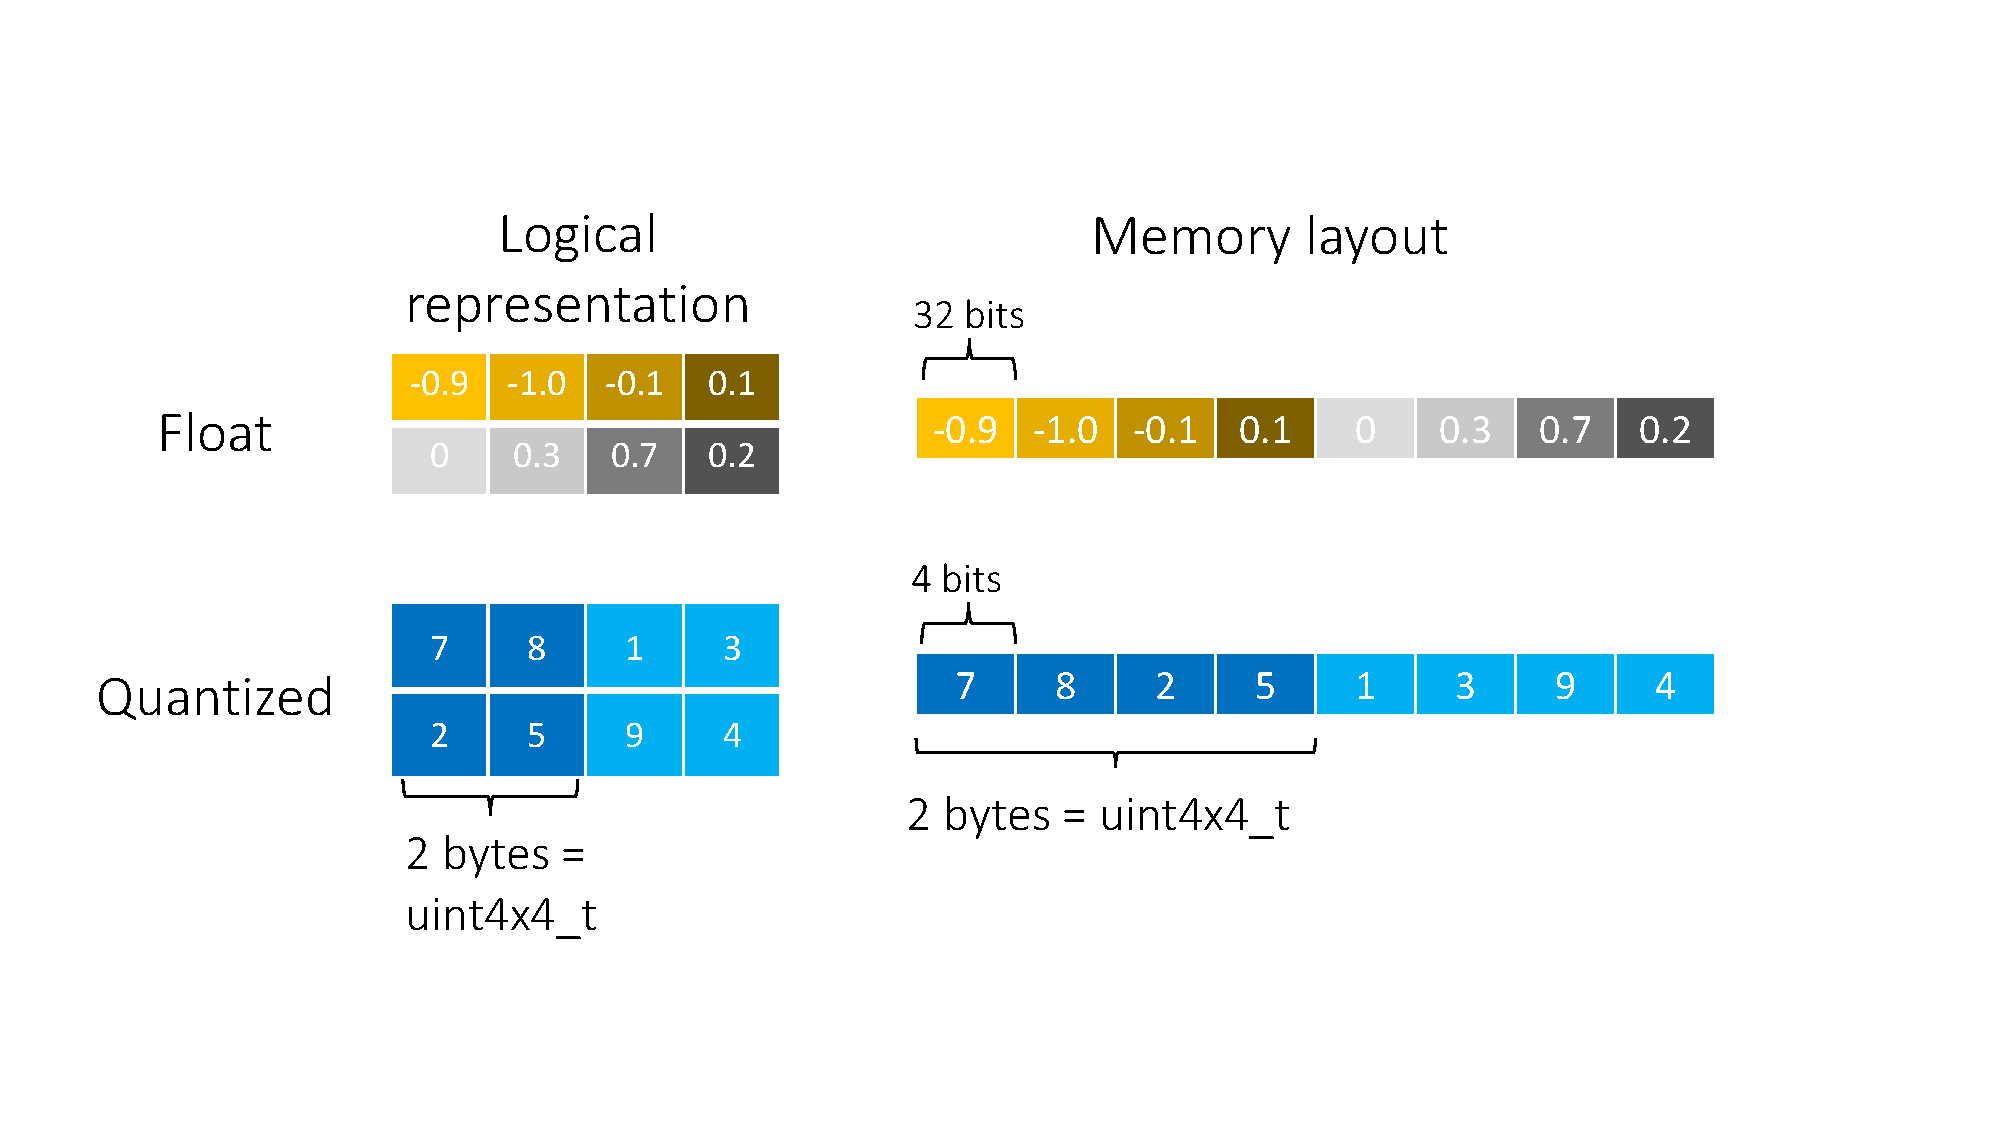
\includegraphics[scale=0.3]{figures/uint4x4_t.pdf}
  \caption{\label{fig:uint4x4_t}Logical and memory layouts of a weight matrix and its corresponding 4-bits quantized version stored as a matrix of $uint4x4\_t$. Cells that share the same color are stored in the same data structure. }
\end{figure}


\mypar{Operation count optimization}
The first optimization we present concerns the reduction of redundant computation. Using simple linear algebra, we can rewrite \cref{eq:qmmm} as:
\begin{align}\label{eq:qmmm_smart}
\begin{split}
\mathcal{Q}(\mathbf{L}) \mathcal{Q}(\mathbf{R}) = \Delta(\mathbf{L}) \Delta(\mathbf{R}) ( \tilde{\mathcal{Q}}(\mathbf{L}) \tilde{\mathcal{Q}}(\mathbf{R}) - z(\mathbf{L}) \mathbf{J} \tilde{\mathcal{Q}}(\mathbf{R}) + \\
- z(\mathbf{R}) \tilde{\mathcal{Q}}(\mathbf{L}) \mathbf{J} +  z(\mathbf{L}) z(\mathbf{R}) \mathbf{J} \mathbf{J} ).
\end{split}
\end{align}
This formulation of the QMMM makes it easy to see its redundant computation. The result of the product $\mathbf{J} \tilde{\mathcal{Q}}(\mathbf{R})$ contained in the second term inside the parenthesis is a matrix that has all rows equal to each other. In particular the $i^{th}$ term of any such row is the sum of the elements of the $i^{th}$ column of  $\tilde{\mathcal{Q}}(\mathbf{R})$. As a consequence, one can compute such row only once and save computation. In particular, this means we move ops from the inner most loop of the QMMM to the second  inner most loop. Thus, the count of such ops grows quadratically with the size of the weight matrix rather than cubically. A similar reasoning can be applied to the third and fourth term inside the parenthesis.

\mypar{Memory optimization}
Another important optimization of our implementation is related to the efficient use of the memory. In particular, we focus on the inner most loop of the QMMM as it is the most critical when it comes to memory bandwidth.


\mypar{Vectorization}
Finally, a critical aspect of our implementation concerns the vectorization of the code. The gain in performance that can be expected vary depending on what type of data a function operates on. For example, if we consider the functions needed to implement the quantization step, we can expect to observe a gain in performance up to $\times 8$ because an AVX register can operate on $8$ floats simultaneously. On the other hand, when we  consider the QMMM, in principle we can expect a gain in performance up to $\times 16$. This is because, in order to have the representation power that is necessary to compute correctly the dot products that appear in the term $ \tilde{\mathcal{Q}}(\mathbf{L}) \tilde{\mathcal{Q}}(\mathbf{R})$ of \cref{eq:qmmm_smart}, we use 16-bits integers as accumulators. As a consequence, our implementation of quantization and QMMM is divided into sub-functions that try to keep as separate as possible the integer computation from the float computation. Among them,  the most important are:

\begin{itemize}
\item \emph{round-sat}: computes the round and saturation operation used in line 5 of \cref{alg:quantize} and line 2 of \cref{alg:qmmm}.
\item \emph{quantize}: given a weight matrix $\mathbf{A}$ performs the operation necessary to compute  $\tilde{\mathcal{Q}}(\mathbf{A}) $ except for rounding and saturating (e.g. computing $mn$, $mx$, $\Delta(\mathbf{A})$).
\item \emph{qmmm\_kernel}: computes $ \tilde{\mathcal{Q}}(\mathbf{L}) \tilde{\mathcal{Q}}(\mathbf{R})$,or, in other words, the dot products of the inner most loop of the QMMM.
\item \emph{trick}: computes the sum over columns and rows of $\tilde{\mathcal{Q}}(\mathbf{R})$ and $\tilde{\mathcal{Q}}(\mathbf{L})$ respectively. As explained before, this is needed to reduce the overall ops count of QMMM. 
\item \emph{add\_trick}: adds the appropriate element of the row and the columns computed by the \emph{trick} function to the result of the dot product computed by \emph{qmmm\_kernel}.
\end{itemize}
\Cref{tab:cost} summarizes the cost in FLOPS or IOPS of each of the functions above.

\begin{table}
\centering
\begin{tabular}{ c|c } 
 
 Function & Ops count (int or float) \\
 \hline 
 \emph{round-sat} & $5N^2$ FLOPS \\
\emph{quantize} & $7N^2$ FLOPS \\
\emph{qmmm\_kernel} & $2N^3$ IOPS \\
\emph{trick} & $2N^2 + 2N$ IOPS \\
\emph{add\_trick} & $3N^3$ IOPS \\
 \end{tabular}
  \caption{Cost analysis}
\label{tab:cost} 
\end{table}

\lstinputlisting[language=C++, caption={Load of two $uint4x4\_t$ rows.}, label={list:load_row}]{figures/load.cpp}



%Our baseline implementation consists of two parts:
%\begin{itemize}
%\item Scalar quantization
%\item Scalar matrix to matrix multiplication
%\end{itemize}
%
%\textbf{Scalar Quantization: } Our input data \emph{v} is a vector of 32-bit floats that contains the values for an arbitrary matrix of size $\emph{rows} \times \emph{columns} \in \mathbb{N} \times \mathbb{N} $, i.e.\ $ \emph{v} \in \mathbb{R}^{ \emph{rows} \cdot \emph{columns} } \cong \mathbb{R}^{ \emph{rows} \times \emph{columns} } $. We traverse the values in \emph{v} to identify the minimum (\emph{min}) and maximum (\emph{max}) of the vector, i.e. $ \emph{min} = \min_{ i \in \emph{rows} \cdot \emph{columns} } v[i] , \emph{max} = \max_{i \in \emph{rows} \cdot \emph{columns} } v[i] $. Subsequently, given a desired precision $ \emph{p} \in \mathbb{N} $, we compute the size of a cell in our range $[\emph{min},\emph{max}] \subset \mathbb{R}$ via $ \Delta = \frac{ \emph{max} - \emph{min} }{ 2^{\emph{p}}} \in \mathbb{R} $. Finally, due to the importance of the 0 value in Neural Networks, we apply a correction value to ensure that the 0 value is encoded exactly, computed via $ \zeta = \frac{ | min | }{ \Delta } - \lfloor \frac{ | min | }{ \Delta } \rfloor $. Finally, we may encode every value in \emph{v} according to the encoding scheme: $ \emph{q}[i] = \frac{ \emph{v}[i] } {\Delta} + \zeta , i \in [0, \emph{rows}\cdot\emph{columns}] \cap \mathbb{N} $.
%
%\textbf{Scalar matrix to matrix multiplication: } Once the parameter matrix has been quantized, we arrive at a quantized vector $ \emph{q} \in  \left([0, 2^{\emph{p}} - 1]\right)^{ \emph{rows} \cdot \emph{columns} }$. Assuming that our input vectors ($ \emph{x} \in \mathbb{R}^{rows} $), we must now compute $ \emph{q} \emph{x} $. Given that $ \emph{q} = ( \frac{ \emph{v}[i] }{ \Delta} + \zeta )_{i \in \emph{rows}\cdot\emph{columns}} \cdot \emph{x} = \frac{1}{\Delta} \left(  \emph[v] \cdot \emph{x} \right) + \zeta \cdot (1,1,1,...,1,1) $. Moreover, assuming that the input vectors are encoded in compressed format ($\widetilde{{x}}$), we may rearrange the terms as follows: 
%$ \widetilde{{x}}^{T} \cdot \emph{q} = \frac	{1}{\Delta_q \cdot \Delta_x} \left( \emph{x}' \cdot \emph{v} ) + \frac{\zeta_q}{\Delta_x} \emph{x} + \frac{\zeta_x}{\Delta_q} \emph{v} + \zeta_q \cdot \zeta_x \cdot (1,1,1,...,1,1) \right)$.

%Now comes the ``beef'' of the paper, where you explain what you
%did. Again, organize it in paragraphs with titles. As in every section
%you start with a very brief overview of the section.
%
%For this class, explain all the optimizations you performed. This mean, you first very briefly
%explain the baseline implementation, then go through locality and other optimizations, and finally SSE (every project will be slightly different of course). Show or mention relevant analysis or assumptions. A few examples: 1) Profiling may lead you to optimize one part first; 2) bandwidth plus data transfer analysis may show that it is memory bound; 3) it may be too hard to implement the algorithm in full generality: make assumptions and state them (e.g., we assume $n$ is divisible by 4; or, we consider only one type of input image); 4) explain how certain data accesses have poor locality. Generally, any type of analysis adds value to your work.
%
%As important as the final results is to show that you took a structured, organized approach to the optimization and that you explain why you did what you did.
%
%
%Mention and cite any external resources including library or other code.
%
%Good visuals or even brief code snippets to illustrate what you did are good. Pasting large amounts of code to fill the space is not good.
